% This is samplepaper.tex, a sample chapter demonstrating the
% LLNCS macro package for Springer Computer Science proceedings;
% Version 2.20 of 2017/10/04
%
\documentclass[runningheads]{llncs}
%
\usepackage{comment}
\usepackage{graphicx}
\usepackage{amsmath, amsfonts, amssymb} % 数学公式、符号
\usepackage[english]{babel}
\usepackage{graphicx}   % 图片
\usepackage{url}        % 超链接
\usepackage{bm}         % 加粗方程字体
\usepackage{multirow}
\usepackage{booktabs}
\usepackage{setspace}
\usepackage{algorithm,algpseudocode}

\newcommand{\dd}{\mathrm{d}}
% Used for displaying a sample figure. If possible, figure files should
% be included in EPS format.
%
% If you use the hyperref package, please uncomment the following line
% to display URLs in blue roman font according to Springer's eBook style:
% \renewcommand\UrlFont{\color{blue}\rmfamily}

% hongteng added
\usepackage{bm}
\usepackage{color}
\usepackage{subfigure}
\newcommand{\xu}[1]{{\color{red} xu: #1}}

\begin{document}
%
\title{Self-Organized Hawkes Processes\thanks{Supported by organization x.}}

% INITIAL SUBMISSION 
\def\CICAISubNumber{132}  % Insert your submission number here
%\begin{comment}
\titlerunning{CICAI2021 submission ID \CICAISubNumber} 
\authorrunning{CICAI2021 submission ID \CICAISubNumber} 
\author{Anonymous CICAI submission}
\institute{Paper ID \CICAISubNumber}
%\end{comment}
%******************

% CAMERA READY SUBMISSION
\begin{comment}
\titlerunning{Abbreviated paper title}
% If the paper title is too long for the running head, you can set
% an abbreviated paper title here
%
\author{First Author\inst{1}\orcidID{0000-1111-2222-3333} \and
Second Author\inst{2,3}\orcidID{1111-2222-3333-4444} \and
Third Author\inst{3}\orcidID{2222--3333-4444-5555}}
%
\authorrunning{F. Author et al.}
% First names are abbreviated in the running head.
% If there are more than two authors, 'et al.' is used.
%
\institute{Princeton University, Princeton NJ 08544, USA \and
Springer Heidelberg, Tiergartenstr. 17, 69121 Heidelberg, Germany
\email{lncs@springer.com}\\
\url{http://www.springer.com/gp/computer-science/lncs} \and
ABC Institute, Rupert-Karls-University Heidelberg, Heidelberg, Germany\\
\email{\{abc,lncs\}@uni-heidelberg.de}}
\end{comment}
%******************
\maketitle              % typeset the header of the contribution

\begin{abstract}
In this paper, we propose a novel self-organized Hawkes process (SOHP) to model complex event sequences based on extremely few observations.
Motivated by the fact that the complicated global relations among events are often composed of simple local relations, we model the event sequences by a set of heterogeneous local Hawkes processes rather than a single Hawkes process. 
In the training phase, we learn the Hawkes processes with a self-organization mechanism, selecting training sequences adaptively for each Hawkes process by a bandit algorithm.
The reward used in the algorithm is originally defined based on an optimal transport distance. 
Additionally, we leverage the superposition property of the Hawkes process to enhance the robustness of our algorithm to the data sparsity problem. 
We apply our SOHP method to sequential recommendation problems and achieve encouraging performance in various datasets. 

\keywords{Hawkes process \and Self-Organization \and Sequential Recommendation.}
\end{abstract}
%
%
%


\section{Introduction}
Hawkes process (HP) is a powerful mathematical framework for modeling generative mechanisms of event sequences in the continuous-time domain. 
Since it was applied in modeling the patterns of earthquake~\cite{ogata1988statistical}, its ability to capture exogenous fluctuations of events and endogenous triggering patterns between different event types has made it a popular model in many application scenarios, $e.g.$, high frequency finance~\cite{bacry2015hawkes}, and social network~\cite{farajtabar2015back}, etc.


Although Hawkes processes provide competitive solutions to many important problems, their practical applications often suffer from some limitations: 
(i) The interrelation of real-world sequences with many event types usually is complicated. 
It is difficult to model their generative mechanism by a single Hawkes process.
\xu{Real-world sequences may yield different models and the interrelation of the event types within each sequence can be complicated. 
Therefore, it is often difficult to model their generative mechanism by a single Hawkes process.}
(ii) It is hard to learn a Hawkes process with a huge number of event types, and the learning tasks are often unavailable for the cases with extremely few observations. 
\xu{Even in the scenario using a single Hawkes process, the number of event types is often huge while the observations can be extremely few in practice, making the learning task challenging.}
The recommendation system just faces the situation such that it's unpractical to apply simply Hawkes processes into the recommendation system.\xu{Too brief... Make the example more detailed, e.g., point out the fact that each user's purchasing behaviors can be very sparse while the number of items is often very large, and the triggering patterns among items for different users can be various... Anyway, make the example convincing!} 



To address these problems, we propose the self-organized Hawkes processes.
The initial reward is calculated as an optimal transport distance.
\xu{The logical chain between the two sentences above is too loose. The second sentence should explain what the meaning of ``self-organized'' is, and what its principle to help solving the issue above.}
As shown in Figure \ref{fig1}, in each iteration, our model selects $K$ sequences for each Hawkes process according to a bandit algorithm. 
\xu{The content in Figure 1 is much more than what you explained above --- it includes not only the bandit part, but also contains the whole learning and prediction pipeline.}
In this paper, we use the greedy strategy, so our model will sample the $K$ sequences with the probability distribution by the magnitude of the reward.
After learning the superposition of these Hawkes processes, the reward of each sequence will be updated by the maximum likelihood score. 
After multiple iterations, we will pick $K$ sequences with biggest reward as the final set of heterogeneous local Hawkes process for each Hawkes process.

Inspired by the work in \cite{lee2013local} and \cite{lee2014local}, we found the fact that the complex global interrelation between events tend to consist of simple local structures. 
Thus, it's feasible to capture mutual excitation in the complicated event sequences by many local Hawkes processes, which make our method more flexible. 
Meanwhile, the work in \cite{xu2018benefits} verified the improvement by the random strategy on selecting sequences. 
Instead of purely random, however, we make the event sequences belonging to each Hawkes process self-organized with the progress of training, which improve the capacity and interpretability of the model.
In addition, our model enhance the robustness to the data sparsity problem for the benefit from the superposition property of the Hawkes process \cite{xu2018benefits}.
Experiments show that our method achieves higher prediction precision compared with the state-of-the-art model.


\begin{figure}[htbp]
\centerline{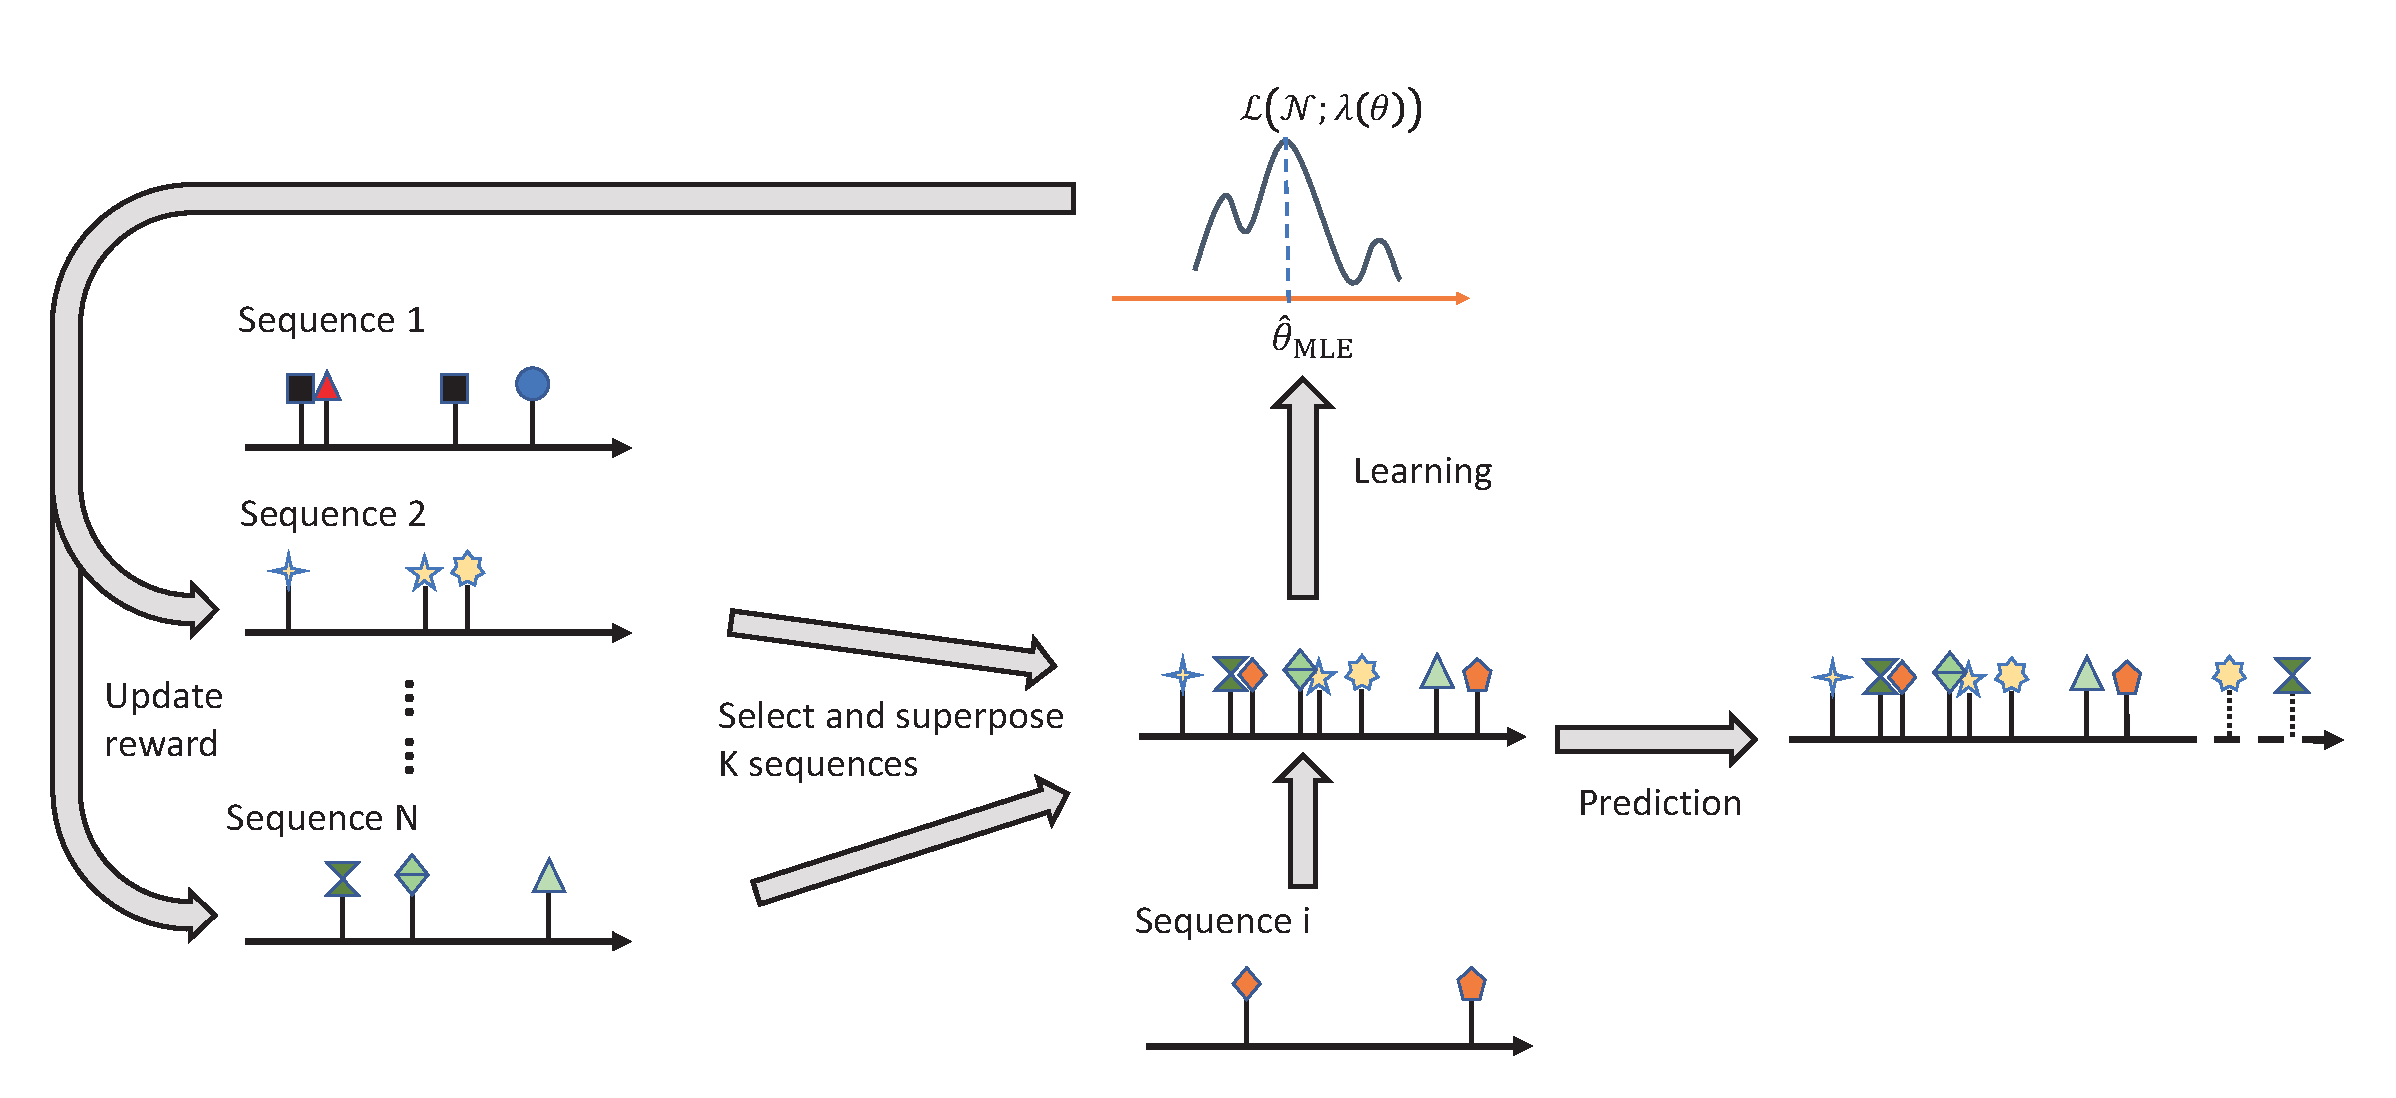
\includegraphics[scale=0.4]{figure1.eps}}
\caption{Self-organized Hawkes processes}
\label{fig1}
\end{figure}

\section{Proposed Model}
\subsection{Continuous-time recommendation based on Hawkes processes}

\subsubsection{Temporal Point Process} 
A temporal point process is a counting process, which can be described as $N = \{ N(t) | t \in [0, T] \}$, where $N(t)$ is the number of events occurring till time $t$, and $[0, T]$ is the time interval of the point process. A multi-dimensional point process with $D$ types is described as $D$ counting processes $\{N_d\}_{d=1}^D$, and $N_d = \{N_d(t) | t \in [0, T]\}$, where $N_d(t)$ is the number of type-$d$ events occurring till time $t$. Given the history, we can define the expected instantaneous happening rate of type-$d$ events as:
\begin{eqnarray}
\begin{aligned}
\lambda_d(t) = \frac{\mathbb{E}[\dd N_d(t)|\mathcal{H}_t^\mathcal{D}]}{\dd t}
\end{aligned}    
\end{eqnarray}
where $\mathcal{H}_t^\mathcal{D}=\{(t_i, d_i)| ti < t, d_i \in \mathcal{D}\}$ is the all historical observation till time $t$.


\subsubsection{Hawkes Processes} 
\xu{Introduce general temporal point process first, give the definitions of basic concepts first (like event sequence, counting process, and conditional intensity function), and then, introduce Hawkes process (a TPP with special intensity functions.)}
A Hawkes process, known as a self-exciting counting process, is a temporal point process with special intensity funcitons.
The expected instantaneous rate of occurrence of type-$d$ event at time $t$ for Hawkes process can be described by a conditional intensity function:
\begin{eqnarray}
\begin{aligned}
\lambda_d(t) = \frac{\mathbb{E}[\dd N_d(t)|\mathcal{H}_t^\mathcal{D}]}{\dd t} = \mu_d + \sum_{t_d < t} \phi_{dd_i} (t, t_i)
\end{aligned}    
\end{eqnarray}
where $\mu_d$ represents the basic happening rates of the type-$d$ event, $\phi_{dd_i} (t, t_i)$ denotes the influence of type-$d_i$ event at time $t_i$ on type-$d$ event at time $t$. 


\xu{Add a paragraph is highlight the good properties of Hawkes process, e.g., modeling the Granger causality among events explicitly, the superposition property, etc. }

Hawkes process is designed to model the self- and mutually-triggering patterns (or the Granger causality) hidden in event sequences explicitly. Additionally, with the superposition-based learning strategy of Hawkes process, we can obtain the tighter bound of excess risk \cite{xu2018benefits} and improve the robustness to the short event sequences.

\xu{You don't have to introduce all learning strategies. If you use MLE, just explain it.}
\subsubsection{Learning} Given a historical event sequence $\mathcal{H}$, we can learn the Hawkes process by Maximum Likelihood Estimation (MLE)
\begin{eqnarray}
\begin{aligned}
\min_{\lambda} \ -\log \mathcal{L}(N;\lambda) + \alpha \mathcal{R}(\lambda) 
\end{aligned}    
\end{eqnarray}

where $\mathcal{L}(\cdot)$ is the  maximum likelihood function. In temporal point process, it can be computed as
\begin{eqnarray}
\begin{aligned}
\mathcal{L}(N;\lambda) = \prod_{(d_i, t_i) \in N} \lambda_{d_i}(t_i) \times \exp \left( - \int \lambda(s) \dd s \right)
\end{aligned}    
\end{eqnarray}

And $\mathcal{R}(\cdot)$ represents the regularization term. This method applies the idea that the observed events are most probable and updates parameters to maximize the likelihood of the observed events. 

\subsubsection{Prediction} 
\xu{Give the general idea about how to make prediction of future events. Then, take sequential recommendation as an example, formulating a recommender based on Hawkes process}

After the conditional intensity function is obtained, we could predict the type of next event in the future. Given a time interval $\Delta t$, the probability of each type of event could be computed by:
\begin{eqnarray}
\begin{aligned}
p(d | t+\Delta t, \mathcal{H}_t) = \frac{\lambda_d(t+\Delta t)}{\lambda (t+\Delta t)}\label{eqn5}
\end{aligned}    
\end{eqnarray}

Next, we will formulate a recommender based on Hawkes process.
For a user $u$, we denote $N_t^{u}=\{(c_i^u, t_i^u)| t_i^u<t\}$ as her purchasing behaviors till time $t$, where $c_i^u\in\mathcal{C}$ is the item she bought at time $t_i^u$. 
Assume that her behaviors yield a multivariate Hawkes process of the items, her expected instantaneous purchasing rate at time $t$ ($i.e.$, her conditional intensity function) is 
\begin{eqnarray}
\begin{aligned}
\lambda_{c}^u(t) = \mu_c + \sum_{t_i^u < t} a_{cc_i^u}\kappa(t- t_i^u),~\forall~c\in\mathcal{C}, \label{eqn6}
\end{aligned}    
\end{eqnarray}
where $\bm{A}=[a_{c\cdot}]\in\mathbb{R}^{|\mathcal{C}|\times |\mathcal{C}|}$ is the infectivity matrix capturing the triggering patterns among the items, $\bm{\mu}=[\mu_c]\in\mathbb{R}^{|\mathcal{C}|}$ represents the basic happening rates of the items, $\kappa(\cdot)$ is the kernel function. 

Plugging (\ref{eqn6}) into (\ref{eqn5}),
\begin{eqnarray}
\begin{aligned}
p(c| t+\Delta t, N_t^u) = \frac{\mu_c + \sum_{t_i^u < t} a_{cc_i^u}\kappa(t- t_i^u)}{\left\|\bm{\mu} \right\|_1 + \sum_{c \in \mathcal{C}} \sum_{t_i^u < t} a_{cc_i^u}\kappa(t- t_i^u)}\label{eqn7}
\end{aligned}    
\end{eqnarray}
It's pratical to recommend items for each user by (\ref{eqn7}).

\subsection{Self-organized Hawkes processes}
\xu{Introduce SOHP}

\xu{This paragraph is recalling your MOTIVATIONS in the sequential recommendation scenarios, which is VERY important. You method is driven by not only the sparsity of events but also the huge number of items. 
Inspired by existing local low-rank/collaborative recommendation models (Guy's work, add citation here), you proposed the self-organized Hawkes process below. Pls polish this paragraph.}

The recommendation system usually need to be faced with a large amount of users with an extremely short purchasing history and the huge number of items, which makes it hard to handle with these problems via modelling a single Hawkes process. To address these problems, inspired by the work in \cite{lee2013local} and \cite{lee2014local}, we proposed the self-organized Hawkes processes, which will be described with details in next section. 

\xu{After introducing your motivation, you give superposed Hawkes process as a potential solution and highlight. That's fine. And you should add one or two sentences in the end to point out your learning task --- not only learning multiple Hawkes processes, but also learning a policy to organize their training event sequences. Formulate your learning tasks mathematically! e.g., the MLEs of the Hawkes process with a learnable policy. Try to MERGE the content of section 3.1 into this subsection.}

The work in \cite{xu2018benefits} verified the improvement of the superposition by the random strategy on selecting sequences. 
However, the distinction between sequences varies with the length of sequences. When the sequence length is short and the difference between the sequences is small, the random algorithm can make up for the information missing. When the sequence length is long, the difference between the sequences is large, and random superposition will make the information confusion caused by the distinction cover up the information compensation, where the random algorithm is not suitable to apply. 

For these reasons, we apply the bandit strategy to select training event sequences in this model. In addition, the policy is a offline strategy, which means the set of local sequences decided by a bandit algorithm before learning will be unchanged in the training phase. Thus, it's necessary to design a measurement scheme of similarity of training event sequences.

Suppose the set of real-world event sequences is defined as $\mathcal{N} = \{N^u\}_{u \in |\mathcal{U}|}$. we design the objective function of the bandit algorithm as:
\begin{eqnarray}
\begin{aligned}
\max \sum_{u \in |\mathcal{U}|} \max_{\mathcal{N}' \subset \mathcal{N}} \mathcal{L}(N^u \cup \mathcal{N}'; \lambda)
\end{aligned}    
\end{eqnarray}

where $\mathcal{L}(\cdot)$ is the maximum likelihood function, $\mathcal{N}'=\{N^{s_1};\ldots;N^{s_K}\}$ denotes the set of the most similar sequences for sequence $u$, and $\lambda$ is the intensity function learning from $N^u \cup \mathcal{N}'$. We regard $\mathcal{L}(\cdot)$ as the reward of choices $\mathcal{N}'$ in bandit algorithm, which measures matching degree of the training event sequences.

\xu{After give the task. Add a paragraph to mention the potential advantage  of solving this task.}


In the learning task, we regard the maximum likelihood function maximizing the likelihood of the observed events as the measurement of the set of heterogeneous Hawkes process, which not only improves the interpretability of the model, but also enhances the results in the subsequent experiments.



\section{Learning Algorithm}
\xu{Give the details of your algorithms and analyze its complexity and other properties.}

\subsection{A reward-augmented bandit algorithm}

Suppose the set of real-world event sequences is defined as $\mathcal{N} = \{N^u\}_{u \in |\mathcal{U}|}$. Then, the steps of bandit algorithm are shown in Algorithm 1. The computational complexity of the algorithm is $\mathcal{O}(|\mathcal{U}|^2 L)$ due to $|\mathcal{U}| \gg K$. This algorithm reduces the computational complexity of learning Hawkes process. In each iteration, we only learn the superposition of K sequences, and the number of event types is much less than the total number of that, which greatly reduced the dimension of Hawkes process.

In Algorithm 2, with the benefit matrix $B$ obtained in Algorithm 1, we select $K$ sequences $\{N^{s_1};\ldots;N^{s_K}\}$ of the most similar ones and superpose them for each sequence $N$, respectively. After learning that, instead of leveraging the intensity function with parameter $\bm{\theta}_{\mathcal{N}'}$ to predict, we update the $\bm{\theta}$ with  $\bm{\theta}_{\mathcal{N}'}$. Until all the sequences have been traversed, we use $\bm{\theta}$ to predict. The deficiency of the former is that only items appearing in the $K$ sequences will be recommend, where the algorithm degenerates to the k-nearest neighbors algorithm \cite{fix1985discriminatory}.


\subsection{Distance between event sequences}

\begin{figure}[htbp]
\centerline{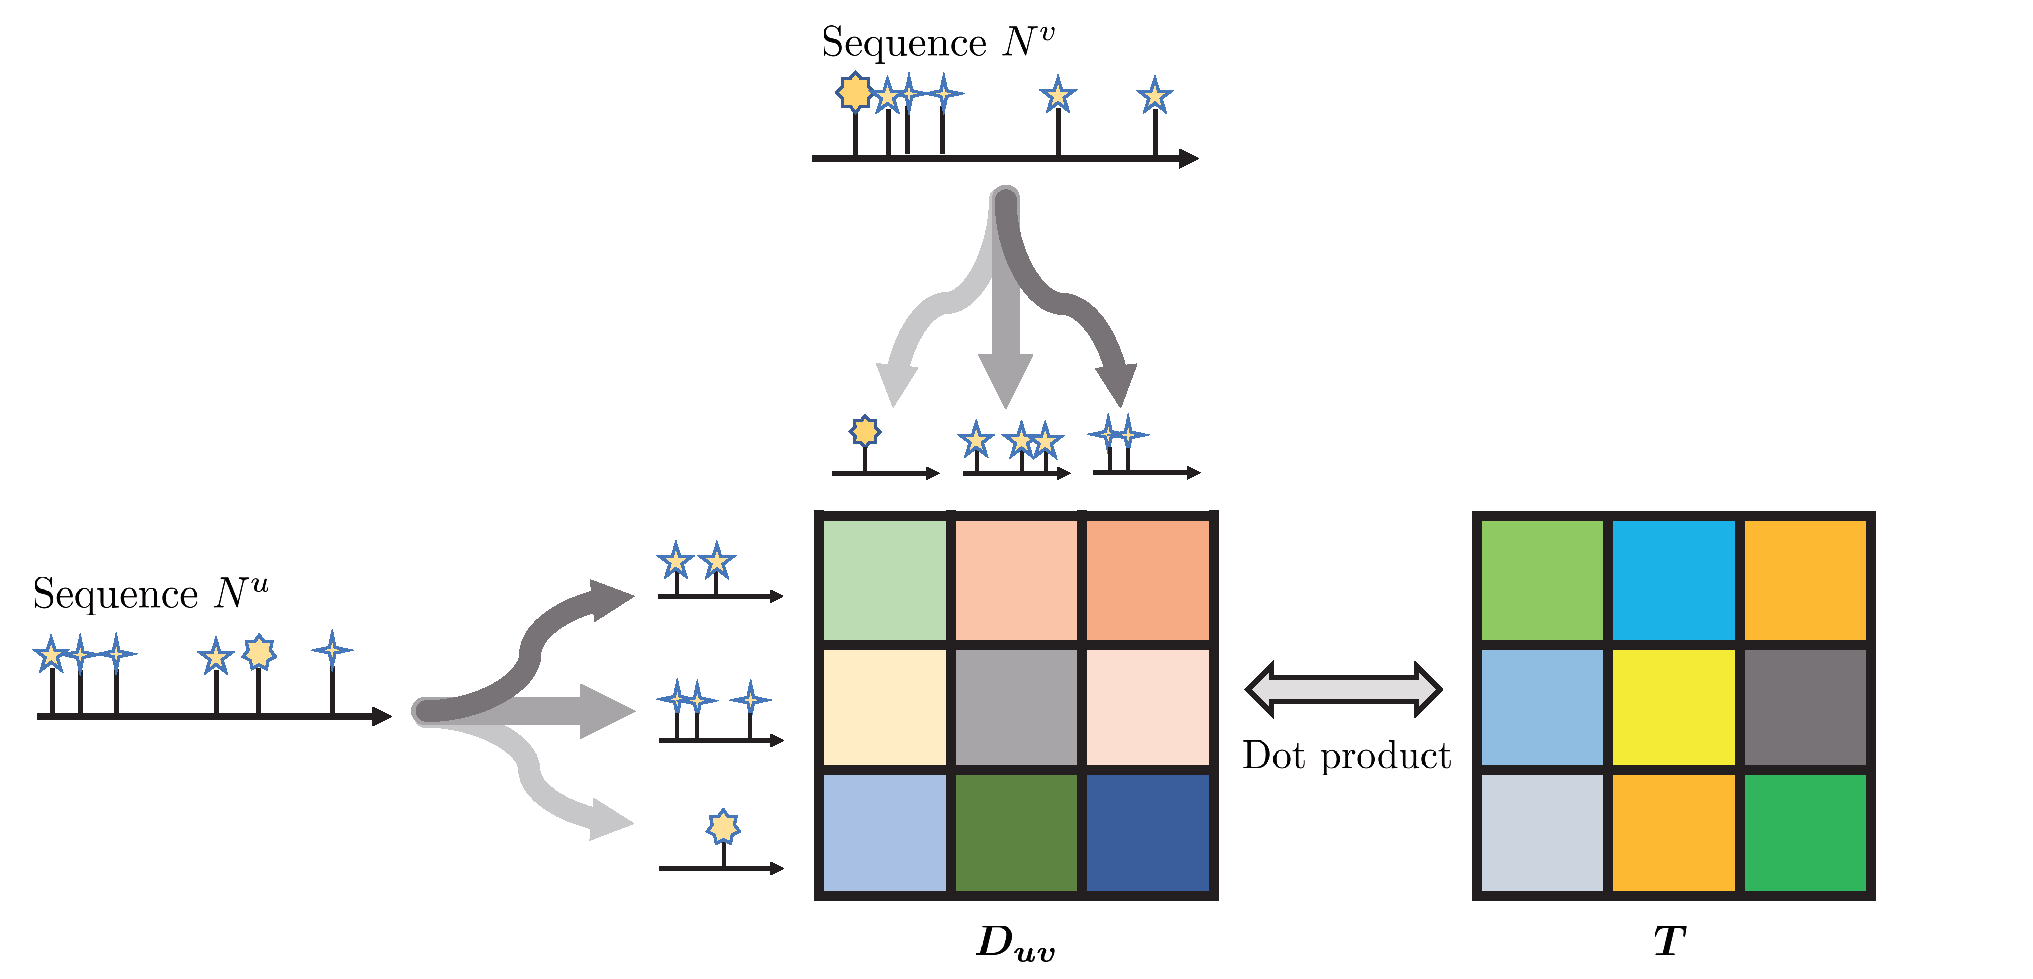
\includegraphics[scale=0.4]{figure2.eps}}
\caption{The optimal transport distance}
\label{fig2}
\end{figure}

\xu{Add a figure to illustrate the computation of the reward.}
The bandit algorithm faces the challenge of the combinatorial explosion of neighbors when calculating the initial benefit. Its computational complexity is $\mathcal{O}(|\mathcal{U}|^{K+1} / K!)$ due to that each user needs to be selected at least once, and each iteration needs to select $K$ neighbors. To solve this, we calculated the optimal transport distance between the purchase sequences for every two users as the initial benefit for each user in the bandit algorithm, as shown in Figure \ref{fig2}.

For $N^u=\{N_i^u \}_{i \in \mathcal{V}_u}$ and $N^v=\{N_j^v\}_{j \in \mathcal{V}_v}$, where $\mathcal{V}_u$ and $\mathcal{V}_v$ are respectively the sets of items purchased by user $u$ and $v$. Here, we leverage optimal transport distance to calculate:
\begin{eqnarray}
\begin{aligned}
d(N^u, N^v) 
& := \min_{\bm{T} \in \prod (\frac{1}{|\mathcal{V}_u|} \bm{1}_{|\mathcal{V}_u|}, \frac{1}{|\mathcal{V}_v|} \bm{1}_{|\mathcal{V}_v|})} \sum_{i \in \mathcal{V}_u, j \in \mathcal{V}_v} T_{ij} d(N_i^u, N_j^v)\\
&= \min_{\bm{T} \in \prod (\frac{1}{|\mathcal{V}_u|} \bm{1}_{|\mathcal{V}_u|}, \frac{1}{|\mathcal{V}_v|} \bm{1}_{|\mathcal{V}_v|})} \langle \bm{D}_{uv}, \bm{T} \rangle 
\end{aligned}    
\end{eqnarray}

where $\bm{T}$ is the optimal transport matix which measures the correlation between different event types, $\bm{D}_{uv}=[d(N_i^u, N_j^v)] \in \mathbb{R}^{|\mathcal{V}_u| \times |\mathcal{V}_v| }$ calculates the distance for sequence $N^u$ and $N^v$, and $d(N_i^u, N_j^v) = \frac{1}{T} \int_0^T|N_i^u(t) - N_j^v(t)| \dd t$ represents the discrepancy between the sequence of the item $i$ and that of the item $j$.

This reduces the computational complexity to $\mathcal{O}(M^2 |\mathcal{U}|^2)$, where $M$ denotes the average length of sequences.

\xu{Add a paragraph to introduce the inference/prediction method after learning the SOHP model, e.g., inferring the global infectivity matrix by superposing the local ones. Add a figure to illustrate the inference step.}

We can infer the global infectivity matrix by superposing the local ones obtained in learning the self-organized Hawkes process for each sequence. As shown in Figure \ref{fig3}, each dimension of the local infectivity matrix is added to the corresponding dimension of the  the global ones. Then, it's practical to predict the future behavior of each user by the global infectivity matrix.

\begin{figure}[htbp]
\centerline{\includegraphics[scale=0.5]{figure3.eps}}
\caption{The inference method}
\label{fig3}
\end{figure}

\begin{algorithm}[t]
\caption{Similarity based on Bandit algorithm} 
\hspace*{0.02in} {\bf Input:}
Event sequences $\mathcal{N}=\{N^u\}_{u \in \mathcal{U}}$, distance matrix of sequences $V=[d(N^u, N^v)] \in \mathbb{R}^{|\mathcal{U}| \times |\mathcal{U}|}$, iterations $L$, number of neighbors $K$, learning rate $\alpha$ \\
\hspace*{0.02in} {\bf Output:} 
benefit matrix $B \in \mathbb{R}^{|\mathcal{U}| \times |\mathcal{U}|}$
\begin{algorithmic}[1]
\For{$u = 1:|\mathcal{U}| $} 
    \State $B_{u,:} = \max (V_{u,:}) - V_{u,:}$
    \For{$l=1:L$}
        \State Set $\bm{p}=[\frac{B_{u,1}}{\sum_i B_{u,i}};\ldots;\frac{B_{u,|\mathcal{U}|}}{\sum_i B_{u,i}} ]$
        \State Sample $K$ sequences $\{N^{s_1};\ldots;N^{s_K}\}$ from $\mathcal{N}$ with $\bm{p}$
        \State Initialize $\mathcal{N}' = \{N^u\} \cup \{N^{s_1};\ldots;N^{s_K}\}$
        \State Learn MHP($\theta$) from $ \mathcal{N}' $
        \For{$k=s_1:s_K$}
        \State $B_{u,k} = B_{u,k} + \alpha \mathcal{L}(N';\theta)$
        \EndFor
    \EndFor
\EndFor
\end{algorithmic}
\end{algorithm}


\begin{algorithm}[t]
\caption{Learning self-organized Hawkes processes} 
\hspace*{0.02in} {\bf Input:}
Event sequences $\mathcal{N}=\{N^u\}_{u \in \mathcal{U}}$, benefit matrix $B \in \mathbb{R}^{|\mathcal{U}| \times |\mathcal{U}|}$, number of neighbors $K$ \\
\hspace*{0.02in} {\bf Output:} 
Parametes $\bm{\theta} = \{\bm{\mu};\bm(A)\}$
\begin{algorithmic}[1]
\State Initialize $\bm{\theta}$ with zero
\For{$u = 1:|\mathcal{U}| $} 
    \State Set $s_1, \ldots, s_K$ as the indices of the top $K$ maximums of $B_{u,:}$
    \State Set $\mathcal{N}' = \{N^u\} \cup \{N^{s_1};\ldots;N^{s_K}\}$
    \State Learn MHP($\bm{\theta}_{ \mathcal{N}' }$) from $ \mathcal{N}' $
    \State Superpose $\bm{\theta}_{ \mathcal{N}' }$ to $\bm{\theta}$ 
\EndFor
\end{algorithmic}
\end{algorithm}


\section{Related Work}
\xu{Enumerate related works and analyze their pros and cons.}
\subsection{Sequential recommendation}

By modeling the sequential behaviors from user historical records, sequential recommendation predicts future interests and recommend items. Besides the shopping recommendation, sequential recommendation has also been widely used in various application scenarios, such as web recommendation \cite{zhang2015task},  music recommendation \cite{chen2012playlist}, and Point-of-Interest recommendation \cite{cheng2013you}\cite{feng2015personalized}, etc.

These years, many cutting-edge techniques have been applied into the sequential recommend, $e.g.$, FPMC\cite{rendle2010factorizing} integrated matrix factorization and Markov chains, HRM\cite{wang2015learning} regarded representation learning as latent factors, they modeled the sequential behavior patterns via every two contiguous historical records. DREAM\cite{yu2016dynamic} based on recurrent neural network (RNN) learnt the global sequential behavior patterns.

These models all captured the contiguous behavior information without taking time interval between them into considering. Instead, we leverage the time stamps of every behavior to calculate efficiently the mutual effect of them.


\subsection{Hawkes process}

Because of its effective modeling of the interaction in real-world event sequences, Hawkes process has been widely used in many scenarios, such as high frequency finance \cite{bacry2015hawkes}, and fake news mitigation \cite{farajtabar2017fake}. Meanwhile, many variants based on Hawkes process have been researched and developed, such as Hawkes process with self-attention \cite{zhang2019self} \cite{zuo2020transformer}, Hawkes process with Granger causality graph \cite{xu2016learning}. Recently, the superposition of Hawkes process has been verified to be effective in both theory and experiments \cite{xu2018benefits}. The model, however, applied a random algorithm to select sequences, where we demonstrate that a bandit algorithm is more valid.



\subsection{Bandit problem}

Bandit problem, $i.e.$, the multi-armed bandit problem denotes a problem where we need to make choices to maximize expected gain under some constraints\cite{robbins1952some}. These years, more bandit algorithms have been proposed, such as Upper Confidence Bounds algorithm \cite{li2010contextual} \cite{chu2011contextual} \cite{bouneffouf2019optimal}, adaptive epsilon-greedy strategy based on Bayesian ensembles \cite{gimelfarb2020epsilon}, and behavior constrained Thompson Sampling \cite{balakrishnan2019incorporating}, etc.
In this paper, we make an attempt to apply the bandit algorithm into superposition of Hawkes process.


\section{Experiments}
\subsection{Implementation details}
\xu{Introduce the data, the baselines, the evaluation criteria, and the configurations of hyperparameters in your work.}

\subsubsection{Datasets} 
We experiment on the Amazon review dataset \cite{he2016ups} \cite{mcauley2015image}. 
This dataset contains product reviews from Amazon spanning May 1996 - July 2014. 
We select five product categories to evaluate our model, including "Instant Video", "Musical Instruments", "Video Games", "Baby" and "Patio, Lawn and Garden".
To be specific, we preprocess the dataset as follows.
We select those items with more than 40 reviews. Then, their users need to satisfy three conditions: (i) the ratings they gave to these items are bigger than 4; (ii) there are at most 3 reviews spanning January 2014 - April 2014; (iii) there are at least 1 review from April 2014 to July 2014.
The statistics of the final datasets are shown in Table \ref{tab1}.
After learning the behaviors of users from January 2014 to April 2014, our model needs to predict items for them from April 2014 to July 2014.

\begin{table}[htbp]
\centering
\caption{Statistics of our datasets}
    \begin{tabular}{c|c|c|c}
    \hline
    \hline
    Categories & \#Users & \#Items & \#Ratings \\
    \midrule
    Musical Instruments & 471   & 678   & 1218 \\
    Baby  & 1979  & 2134  & 6070 \\
    Video Games & 2142  & 2104  & 6126 \\
    Garden & 1812  & 2064  & 4976 \\
    Instant Video & 5948  & 1344  & 15470 \\
    \hline
    \end{tabular}%
\label{tab1}%
\end{table}%
  

\subsubsection{Baselines}
We adopt the following state-of-the-art models as baselines for comparison:
\begin{itemize}
    \item \textbf{SVD} Singular value decomposition, a classical method from linear algebra is getting popular in recommender systems.
    \item \textbf{kNN} K-nearest neighbors algorithm, a non-parametric classification and regression method. We adopt the user-based kNN in the experiments.
    \item \textbf{BPR} Bayesian personalized ranking \cite{rendle2012bpr}, a popular method for top-N ranking recommendation. 
    \item \textbf{SLIM} Sparse linear method \cite{ning2011slim}, a simple and effective method for top-N recommendation.
    \item \textbf{FPMC} Factorized personalized Markov chains \cite{rendle2010factorizing}, one of the stat-of-the-art models for sequential recommendation based on matrix factorization and Markov chains. Each item is regarded as a basket in this model.
\end{itemize}

\subsubsection{Evaluation methods} For each model, the generated recommendation list for user $u$ is defined as $R^u = \{r_1^u,\ldots,r_N^u \}$, where $r_i^u$ is ranked at the $i$-th position. Suppose the real set of her interacted items is $T^u$, and the number of users is $M$, we thus use the following measures for evaluation:

\begin{align*}
P@N &= \frac{1}{M}\sum_u P_u@N = \frac{1}{M} \sum_u \frac{|R_u \cap T_u|}{|R_u|}\\
R@N &= \frac{1}{M}\sum_u R_u@N = \frac{1}{M} \sum_u \frac{|R_u \cap T_u|}{|T_u|}\\
F_1@N &= \frac{1}{M}\sum_u F_{1u}@N = \frac{1}{M} \sum_u \frac{2 \cdot P_u@N \cdot R_u@N}{P_u@N + R_u@N}
\end{align*}    




\subsubsection{Parameter settings}

When implementing our method, the number of iterations $L$ for each user is set as $20$ and the learning rate $\alpha$ is set as $0.1$. We primarily set
the number of neighbors $K=10$, and the effect of setting different $K$ is studied in the experiments.
When learning the superposition of Hawkes processes, we empirically set the decay $\beta=0.00003$ and use no regularization term.
For each user, $10$ items need to be recommended.



\subsection{Comparisons and analysis}
\xu{Show your experimental results here. Besides direct comparisons, try to add more analytic experiments to demonstrate the rationality of the method --- show the necessity of using self-organized Hawkes process model and its learning algorithm.}

\xu{Table 1. Comparison with existing methods on recommendation accuracy.}

\xu{Runtime comparison between your method and other Hawkes-based variants.}

\xu{The influence of the number of neighbors for each dataset.}

\xu{The influence of different reward designs.}

\begin{table}[htbp]
    \centering
    \caption{Summary of the performance for baselines and our model}
    \resizebox{.95\columnwidth}{!}{
      \begin{tabular}{c|ccc|ccc|ccc|ccc|ccc}
      \hline
      Datasets & \multicolumn{3}{c|}{Musical Instruments} & \multicolumn{3}{c|}{Baby} & \multicolumn{3}{c|}{Video Games} & \multicolumn{3}{c|}{Garden} & \multicolumn{3}{c}{Instant Video} \\
      \hline
      \hline
      Measures@10(\%) & P     & R     & F1    & P     & R     & F1    & P     & R     & F1    & P     & R     & F1    & P     & R     & F1 \\
      \hline
      SVD   & 0.106 & 1.061 & 0.193 & 0.121 & 0.735 & 0.207 & 0.065 & 0.498 & 0.113 & 0.055 & 0.395 & 0.094 & 0.126 & 1.052 & 0.221 \\
      kNN   & 0.382 & 2.671 & 0.649 & 0.389 & 2.513 & 0.638 & 0.661 & 4.915 & 1.163 & 0.237 & 1.751 & 0.405 & 0.817 & 6.901 & 1.435 \\
      BPR   & 0.467 & 3.750 & 0.811 & 0.389 & 2.469 & 0.635 & 0.658 & 4.864 & 1.112 & 0.110 & 0.762 & 0.185 & 0.859 & 7.049 & 1.503 \\
      SLIM  & 0.212 & 1.351 & 0.347 & 0.111 & 0.712 & 0.180 & 0.499 & 3.595 & 0.835 & 0.242 & 1.544 & 0.401 & \textbf{1.333} & \textbf{11.428} & \textbf{2.351} \\
      FPMC  & 0.594 & 4.193 & 1.006 & 0.283 & 1.912 & 0.470 & 0.556 & 3.799 & 0.927 & 0.171 & 1.117 & 0.285 & 0.931 & 7.413 & 1.622 \\
      Our methods(random) & 0.361 & 2.406 & 0.604 & 0.258 & 1.734 & 0.432 & 0.317 & 2.037 & 0.525 & 0.199 & 1.350 & 0.331 & 0.933 & 7.406 & 1.623 \\
      Our methods & \textbf{0.658} & \textbf{5.149} & \textbf{1.138} & \textbf{0.389} & \textbf{2.640} & \textbf{0.651} & \textbf{0.700} & \textbf{5.108} & \textbf{1.180} & \textbf{0.248} & \textbf{1.801} & \textbf{0.436} & 0.999 & 7.911 & 1.738 \\
      \hline
      \hline
      \end{tabular}%
    }
    \label{tab2}%
  \end{table}%
  
\begin{figure}[htbp]
\centerline{\includegraphics[scale=0.4]{figure4.png}}
\caption{Performance of our model under different number of neighbors $K$. }
\label{fig4}
\end{figure}

Table 2 summarizes the performance for baselines and our model on the five categories listed in Table 1. For all categories except "Instant Video", the proposed self-organized Hawkes process model achieves better performance than the best baselines. 
Specifically, in the category "Musical instrument", the result of our model is $13\%$ higher than that of the best baseline ($i.e.$, FPMC), and the difference would be up to $48\%$ by tuning $K$ in the subsequent experiments. The results indicates the availability of our model for sequential recommendation.

we are curious about whether and how the number of local heterogeneous Hawkes process affects recommender.
To do so, we analyze the influence of setting different $K$ which defines the number of the training event sequences for each sequence.
Specifically, we study the performance of our model on F1@10
by tuning $K$ in the range of $\{2,5,10,20,50,100\}$. Results are
shown in Figure \ref{fig4}. 

For the categoies "Musical Instruments" and "Baby", as the increase of $K$, the performance of them gets better. At this moment, the model learns more popular interests and will be more inclined to recommend the most popular items. For the category "Musical Instrument", there are fewer kinds of instruments, and the standard for each instrument is fixed, so the public tends to purchase more expensive one according to the principle of "the more expensive the better". In the case of the category "Baby", babies can't comment on the items, so parents tend to choose the most popular products.

For the categoies "Video Games" and "Garden", when the local structures are simple, the performance increases drastically, and the best result is achieved when $K \  \approx \ 10 $. However, when the number of neighbors continues to rise, the performance goes down. This phenomenon is easy to understand. When there are fewer training event sequences, local structures provide less information, which make it difficult to capture global relations. However, when there are too many neighbors, our model will tend to recommend the most popular items, which isn't suitable for these datasets.

For the category “Instant Video”, however, we find that our model is inferior to the SLIM method. According to our analysis, a possible reason for this phenomenon is that for most users, their choice of instant video tend to be influenced by Amazon's recommendations or the most popular video list, which may not be suitable for sequential recommendation. Evidence supporting this explanation is that FPMC which is also a sequential recommendation model, has poor performance.



\section{Conclusion}
In this paper, we proposed a framework leveraging the superposition of Hawkes processes integrated with bandit algorithm for sequential recommendation. To do so, we design the reward of the Bandit algorithm, and exert the greedy strategy to update the reward iteratively. What's more, we analyse the computation complexity and properties of this model. In the future, we plan to design new formulation of rewards and update rewards with other strategies. Additionally, we will make attempts to apply self-adaptive number of training event sequences for each sequence.

\bibliographystyle{splncs04}
\bibliography{references}

\clearpage
\newpage



\end{document}
